\chapter{Background}\label{chap:background}
This chapter provides an overview of the basic concepts of object detection and tracking and the steps of an MTMCT system, along with a discussion of its key challenges and issues. It also introduces the basic building blocks of MTMCT. Finally, the datasets and metrics used to evaluate MTMCT systems are explained.

\section{Steps of an MTMCT System}\label{sec:steps_of_an_mtmct_system}
An MTMCT system typically consists of the following steps: detection, feature extraction, data association, and tracking. The steps are only briefly mentioned and described here, exact methods and algorithms are discussed in the chapter~\ref{chap:literature_review}.

\subsection{Detection}\label{subsec:detection}
Detection refers to the process of identifying objects of interest within video frames. This is typically done using a variety of techniques, ranging from traditional image processing methods to deep learning models. The goal of the detection step is to locate and classify objects in the frame, providing a basis for subsequent steps in the MTMCT process.

\subsection{Feature Extraction}\label{subsec:feature_extraction}
Feature extraction involves extracting relevant information from detected objects to facilitate tracking. This can include low-level features such as color, shape and texture, as well as high-level features such as object parts and their spatial relationships, speed, and direction of motion. The features extracted from objects are used to identify and distinguish them from other objects in the scene.

\subsection{Data Association}\label{subsec:data_association}
To understand the data association step, it is necessary to define the following terms:

\begin{itemize}
    \item \textbf{Tracklets:} Short segments of a path of an object captured within the view of a single-camera, formed by connecting successive frame detections.
    \item \textbf{Trajectories:} The complete path of an object over time, often across multiple frames and cameras, created by merging tracklets.
    \item \textbf{Tracks:} Refined trajectories that represent the validated path of an object after correction for inaccuracies and false detections.
\end{itemize}

In the research literature, these terms are often used interchangeably and not always consistently, but for the purposes of this project, the above definitions will be used.

Data association is the process of associating currently detected objects with existing trajectories based on similarities in their features. This is done by comparing the features of detected objects with the features of existing trajectories and assigning the detected objects to the most similar trajectories. This step is critical for maintaining the ID of objects as they move through or even leave and re-enter the scene, which is called re-ID. Typically, the data association step is performed hierarchically: first on a single-camera view (intra-camera), before the trajectories are associated across multiple camera views (inter-camera) and finally optimized globally.

\begin{figure}[ht]
    \centering
    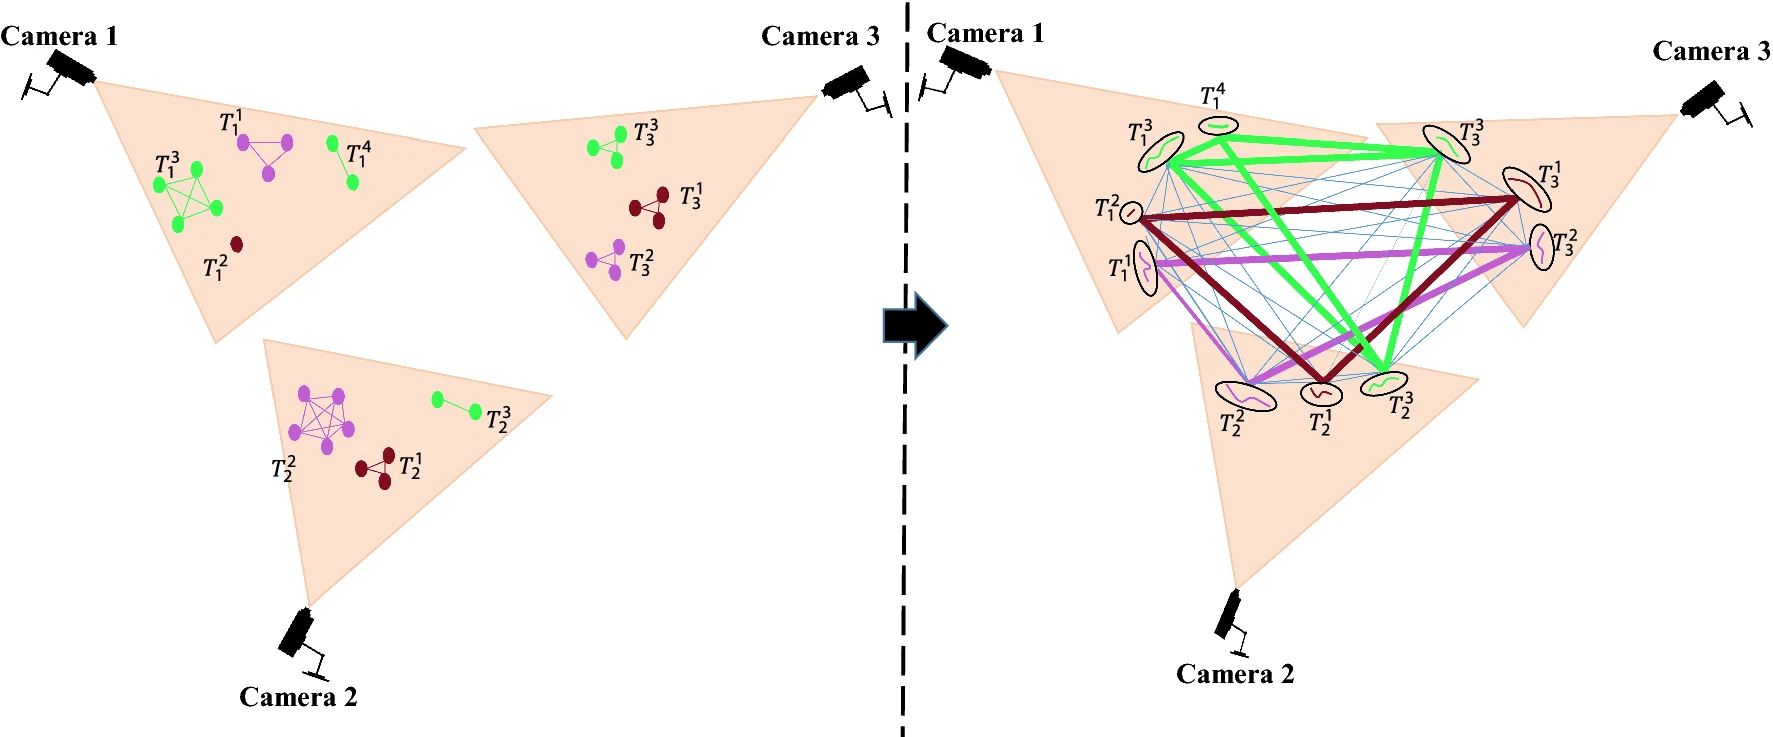
\includegraphics[width=0.75\textwidth]{resources/fig/Tesfaye19-intra_inter_camera_tracking.png}
    \caption{Intra- (left) and inter-camera (right) tracking~\cite[Fig.~1]{Tesfaye19}}\label{fig:intra_inter_camera_tracking}
\end{figure}

The two steps of data association of three non-overlapping camera views are illustrated in Figure~\ref{fig:intra_inter_camera_tracking}. The first step is intra-camera tracking, where the trajectories within the three camera views are associated independently. The second step is inter-camera tracking, where the trajectories are associated across the three camera views and the IDs of the objects are maintained. This simple example can be extended to any number of camera views, overlapping or non-overlapping.

\subsection{Tracking}\label{subsec:tracking}
Tracking refers to the step of maintaining the trajectory of detected objects over time. This involves predicting the future location of an object based on its past movements and updating its trajectory as new observations (tracklets), the next frame of a video, become available. In summary, tracking is responsible for maintaining and managing the trajectories and IDs of objects as they move through the scene and ensuring consistent global IDs across multiple camera views.

\section{Fundamental Concepts}\label{sec:fundamental_concepts}
This section briefly describes the fundamental concepts of MTMCT that are essential for following the progression from basic object tracking methods to advanced MTMCT techniques.

\subsection{Single-Target Single-Camera Tracking}\label{subsec:st_sct}
Single-Target Single-Camera Tracking (STSCT) is the simplest form of object tracking and involves tracking a single target in the FOV of a single-camera. The primary goal of STSCT is to maintain the ID and trajectory of the target as it moves through the FOV of the camera.

\subsection{Multi-Target Single-Camera Tracking}\label{subsec:mt_sct}
Multi-Target Single-Camera Tracking (MTSCT) builds on the principles of STSCT, but introduces the added complexity of dealing with multiple targets in a single-camera view. The goal is to track multiple objects simultaneously while maintaining the ID of each target and avoiding ID switches. This requires sophisticated algorithms that can handle occlusions, interactions between targets, and other challenges that arise especially in crowded scenes.

The evolution from STSCT to MTSCT and ultimately to MTMCT reflects the increasing complexity and ability of tracking systems to handle more complex scenarios. This evolution is made possible by advances in computer vision and machine learning, which provide the tools necessary to overcome the challenges associated with tracking multiple targets across multiple camera views.

\section{Challenges and Issues}\label{sec:challenges_and_issues}
The process of tracking multiple objects across multiple camera views requires careful consideration of several factors that can significantly affect the performance and accuracy of the tracking system. Some of the major challenges and issues faced in MTMCT are discussed in the following subsections.

\subsection{Occlusion}\label{subsec:occlusion}
Occlusion occurs when an object is partially or completely blocked from view, making it difficult to accurately track its position and ID. This can happen when objects overlap or are obstructed by other elements in the scene, such as buildings or trees. Occlusion is a common challenge in crowded environments, such as public spaces and sporting events, where multiple objects are often in close proximity.

\subsection{Varying Lighting Conditions}\label{subsec:varying_lighting_conditions}
Lighting conditions can have a significant impact on the performance of an MTMCT system. Variations in lighting, such as changes in natural light throughout the day or artificial lighting when a tracked object enters a building, can affect the appearance of objects and make it difficult to maintain consistent tracking. The presence of shadows and reflections can also make tracking difficult.

\subsection{Camera Specifications}\label{subsec:camera_specification}
The specifications of the cameras used in an MTMCT system can have a significant impact on its performance. If multiple cameras are used, they may have different specifications:

\begin{itemize}
    \item \textbf{Resolution:} Number of pixels in the image
    \item \textbf{FPS:} Number of frames captured per second
    \item \textbf{FOV:} Area covered by the camera
    \item \textbf{Angle:} Angle from which the camera is capturing the scene
\end{itemize}

This can make it difficult to maintain consistent tracking across different camera views, especially when objects move from one camera to another. Objects can look different when viewed from different cameras, and their size and shape can be distorted. To achieve accurate tracking, the system must account for these variations and correctly align objects across camera views.

\subsection{Uncertainties}\label{subsec:uncertainties}
In an MTMCT system, the number of objects present in the entire camera network, in a single-camera view, and the number of camera views in which a tracked object is present at any given time are all unknown. These uncertainties make it difficult to accurately track objects across multiple camera views.

\section{Datasets}\label{sec:datasets}
Datasets are a fundamental aspect of MTMCT research; they are the resource for training, evaluating, and comparing different tracking methods. A wide variety of datasets exist to meet the needs of research, each presenting unique challenges and scenarios.

Commonly used datasets for training object detectors are:

\begin{itemize}
    \item \textbf{Microsoft COCO (Common Objects in Context):} Comprehensive dataset used for object detection and segmentation. COCO includes a wide variety of objects~\cite{Lin14}.
    \item \textbf{ImageNet:} Large dataset used for image classification and object detection. Object detectors trained on ImageNet are capable of recognizing a wide range of objects~\cite{Deng09}.
\end{itemize}

Beside these datasets, there are several datasets specifically designed for MTMCT research. These datasets are discussed in the subsection~\ref{subsec:datasets_and_challenges}.

\section{Metrics and Evaluation}\label{sec:metrics_and_evaluation}
Evaluating the performance of an MTMCT system is critical to understanding its effectiveness and reliability. In addition to well-known metrics such as accuracy, precision and recall, there are several metrics specifically designed for MTMCT systems. These metrics are discussed in this section.

\subsection{MOTP and MOTA}\label{subsec:motp_mota}
Multiple Object Tracking Precision (MOTP) and Multiple Object Tracking Accuracy (MOTA) are two standard metrics used to evaluate multi-target tracking systems. MOTP measures the accuracy of object localization, while MOTA combines three types of error into a single metric to provide a comprehensive evaluation of tracking performance. Both metrics were introduced by \textcite{Bernardin08} in \citeyear{Bernardin08}.

\begin{equation}
    \label{eq:motp}
    \text{MOTP}=\frac{\sum_{i, t} d_t^i}{\sum_t c_t}
    \quad\text{\cite[Eq.~1]{Bernardin08}}
\end{equation}

The equation \ref{eq:motp} provides a measure of the average error in the estimated positions of the tracked objects. In this equation, \(d_t^i\) is the distance between the predicted position and the ground truth position of object \(i\) in frame \(t\), and \(c_t\) is the number of correctly matched objects (the true positives) in frame \(t\). The distances for all matched objects across all frames are divided by the total number of matched objects across all frames. MOTP ranges from 0 to 1, a lower MOTP value indicates higher precision in object localization.

\begin{equation}
    \label{eq:mota}
    \text{MOTA}=1-\frac{\sum_t (m_t+fp_t+mme_t)}{\sum_t g_t}
    \quad\text{\cite[Eq.~2]{Bernardin08}}
\end{equation}

The equation \ref{eq:mota} combines three types of errors into a single performance measure. In this equation, \(m_t\) is the number of misses (true objects not detected), \(fp_t\) is the number of false positives (false object detections), \(mme_t\) is the number of mismatch errors (ID switches) and \(g_t\) is the total number of true objects present in the frame \(t\). The MOTA score is one minus the sum of all errors divided by the total number of true objects across all frames. MOTA ranges from \(-\infty\) to 1, a higher MOTA value indicates better tracking accuracy.

\subsection{IDF1}\label{subsec:idf1}
The IDF1 score is another important metric for evaluating MTMCT systems. It represents the harmonic mean of identification precision and recall, providing a balanced measure that considers both the ratio of correctly identified detections and the average number of ground truth and computed detections. This metric was introduced by \citeauthor{Ristani16} in their widely referenced paper \citetitle{Ristani16}~\cite{Ristani16}.

\begin{equation}
    \label{eq:idf1}
    \text{IDF}_1 = \frac{2 \times \text{IDTP}}{2 \times \text{IDTP} + \text{IDFP} + \text{IDFN}}
    \quad\text{\cite[Eq.~11]{Ristani16}}
\end{equation}

In equation~\ref{eq:idf1}:

\begin{itemize}
    \item \textbf{IDTP (Identification True Positives):} Represents the number of detections that were correctly identified.
    \item \textbf{IDFP (Identification False Positives):} Represents the number of detections that were misidentified.
    \item \textbf{IDFN (Identification False Negatives):} Returns the number of actual detections that were missed or not identified.
\end{itemize}

The IDF1 metric essentially captures identification precision and recall in multi-object tracking scenarios. The higher the IDF1 score, the better the performance of the tracker in maintaining consistent IDs.

\subsection{MT and ML}\label{subsec:mt_ml}
The Mostly Tracked (ML) and Mostly Lost (ML) metrics are used to evaluate the effectiveness of a tracking system in maintaining consistent trajectories for tracked objects. The metrics published by \textcite{Wu06} in \citeyear{Wu06} are commonly used in benchmarks to evaluate the performance of tracking systems.

MT measures the proportion of ground truth trajectories that are covered by the tracker for at least 80\% of their respective lifetime, indicating the ability of the system to track objects consistently over time. On the other hand, ML measures the proportion of ground truth trajectories that are covered by the tracker for less than 20\% of their respective lifetimes, reflecting the inability of the system to maintain consistent object tracking.

\begin{figure}[ht]
    \centering
    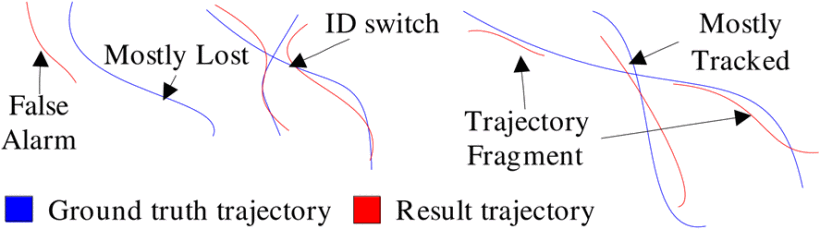
\includegraphics[width=0.75\textwidth]{resources/fig/Wu06-MT_ML.png}
    \caption{MT and ML~\cite[Fig.~5]{Wu06}}\label{fig:mt_ml}
\end{figure}

Figure~\ref{fig:mt_ml} illustrates various scenarios encountered in multi-target tracking evaluations:

\begin{itemize}
    \item \textbf{Ground Truth Trajectory (Blue):} Represents the actual path or movement of an object in the scene.
    \item \textbf{Result Trajectory (Red):} Represents the predicted path of an object by the tracking system.
    \item \textbf{False Alarm:} Points where the tracking system detects an object when there is no object in the ground truth.
    \item \textbf{ID Switch:} An instance where the ID assigned to an object is incorrectly changed during tracking.
    \item \textbf{Trajectory Fragment:} A segment of the resulting trajectory that is shorter than the ground truth, indicating a break or interruption in tracking.
    \item \textbf{Mostly Tracked:} Scenarios where the resulting trajectory closely follows the ground truth trajectory for most of the path of the object (\(\geq 80\%\))
    \item \textbf{Mostly Lost:} Scenarios where the resulting trajectory only briefly aligns or intersects with the ground truth trajectory, indicating that the object was not effectively tracked for most of its path (\(\leq 20\%\)).
\end{itemize}